\documentclass[conference]{IEEEtran}
\IEEEoverridecommandlockouts{}

\usepackage{cite}
\usepackage{amsmath,amssymb,amsfonts}
\usepackage{algorithmic}
\usepackage{graphicx}
\usepackage{textcomp}
\usepackage{xcolor}
\usepackage{hyperref}
%% ODE handling
\usepackage{diffcoeff}
\usepackage{booktabs}
%% The SI units alignment
\usepackage{siunitx}
\def\BibTeX{{\rm B\kern-.05em{\sc i\kern-.025em b}\kern-.08em
    T\kern-.1667em\lower.7ex\hbox{E}\kern-.125emX}}
\begin{document}

\title{Carbon Neutral Greenhouse: A Economic Model Predictive Control Framework for Education
    \thanks{The authors gratefully acknowledge the contribution of the Program to support young researchers under the project Adaptive and Robust Change Detection for Enhanced Reliability in Intelligent Systems. The authors gratefully acknowledge the contribution of the Scientific Grant Agency of the Slovak Republic under the grant 1/0490/23, 1/0297/22 and `1/0691/21'. This research is funded by the Horizon Europe under the grant no. 101079342 (Fostering Opportunities Towards Slovak Excellence in Advanced Control for Smart Industries).}
}

\author{\IEEEauthorblockN{Marek Wadinger, Rastislav F\'{a}ber, Erika Pavlovičov\'{a}, Radoslav Paulen}
\IEEEauthorblockA{\textit{Institute of Information Engineering, Automation, and Mathematics} \\
    \textit{Slovak University of Technology in Bratislava}\\
    Bratislava, Slovakia \\
    \texttt{marek.wadinger@stuba.sk}}
}

\maketitle

\begin{abstract}
    This paper introduces a mathematical model of lettuce growth, integrating key variables such as temperature, light, and humidity, which are influenced by external weather conditions. To account for these external factors, we employ an API to obtain real-time weather forecasts, enabling the dynamic adjustment of greenhouse conditions using a heating system when necessary. The MPC-based approach forecasts future plant growth and energy requirements, enabling precise control over environmental factors. Simulations demonstrate that our approach effectively balances energy consumption with crop yield, resulting in enhanced profitability. The model not only optimizes economic output (€) but also provides a valuable tool for planning and improving greenhouse operations.
    % TODO: doplnit vysledk >> tu chceme hovoriť o vypestovaní šalátu za 1,20€? :D
    By leveraging this model, growers can achieve more efficient, sustainable, and economically viable lettuce production.
    \newline
\end{abstract}
%%
\begin{IEEEkeywords}
    Model Predictive Control, Lettuce Growth Optimization, Greenhouse Energy Management, Precision Agriculture, Economic Yield Optimization
\end{IEEEkeywords}


\section{Introduction}
% - General introduction (why is it important that we do what we do)
Most current farming practices are labor-intensive, seasonal, constrained by irrigation, and dependent on subsidized inputs, leading to significant issues like eutrophication, deforestation, and soil degradation. It also consumes nearly 70\% of global water resources~\cite{Debroy2024}. Greenhouses are pivotal in enhancing agricultural productivity by providing controlled environments that surpass the productivity of open-air cultivation. Despite their benefits, greenhouses face significant challenges due to fluctuating internal temperatures that can lead to crop fading and death. To counteract these issues, it is crucial to improve greenhouse environments through effective climate management, incorporating ventilation or heating to regulate internal conditions and enhance crop yields~\cite{Wu2019}.

% - Concrete introduction (what is the state of the art in the domain)
Solar radiation is fundamental to both plant growth and energy generation in a greenhouse. Key metrics include Global Horizontal Irradiance (\(GHI\)) and Photosynthetically Active Radiation (\(PAR\)), with \(PAR\) being directly responsible for photosynthesis. Recent research has focused on accurately estimating diffuse \(PAR\) and its impact on plant growth, leading to the development of sophisticated models that predict \(PAR\) with varying degrees of accuracy~\cite{Iddio2020, MaLu2022}. In parallel, methods such as adaptive control, nonlinear feedback control, fuzzy control, robust control, and optimum control have been explored for optimizing greenhouse environments, aiming to boost efficiency, resource use, and crop yield. In general, we identify two main types of greenhouse control algorithms: conventional control and optimal control. Conventional control aims to reduce the difference between setpoints and actual measurements. On the other hand, optimal control incorporates factors such as greenhouse dynamics, actuator capabilities, energy consumption, and crop responses into the control strategy

\begin{figure}
    \centering
    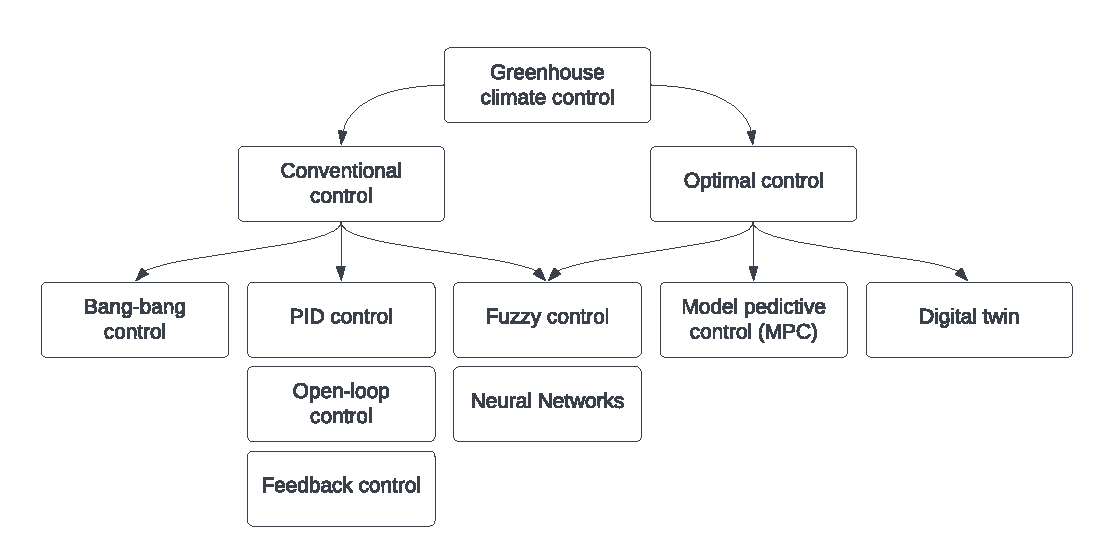
\includegraphics[width=.5\textwidth]{images/flowchart.pdf}
    \caption{A simplified diagram representing greenhouse control algorithms. Image adapted from~\cite{Trepanier2024}.}\label{fig:flowchart}
\end{figure}

Adaptive control adjusts parameters based on real-time feedback~\cite{Tian2022}, while nonlinear feedback control tackles system complexities with advanced algorithms~\cite{Bood2023}. Fuzzy control addresses imprecise data and uncertainties~\cite{smartcities7030055}, and robust control maintains stability despite disturbances~\cite{Zhang2021}. Optimum control aims to fine-tune actions for best outcomes~\cite{Debroy2024, SVENSEN2024108578}. However, these techniques often demand substantial computational power and intricate implementation, additionally, frequent adjustments raise energy consumption and actuator wear.

Consequently, PID controllers remained popular due to their simplicity and effectiveness. IoT and machine learning advancements are also enhancing greenhouse control, with Wang et al.~\cite{Wang2024} combining these technologies with PID for real-time monitoring. Despite improvements, challenges accompany PID control due to the complexity of greenhouse systems requiring multiple controllers and extensive tuning. The process remains time-consuming and dependent on optimization, often without guaranteed optimal results. Therefore, MPC has gained traction in greenhouse climate control~\cite{Hu2022}, however, opting for continuously adjusting parameter setpoints through online optimization on a sample-by-sample basis. This iterative optimization procedure can escalate computational load, thereby complicating system operation.

% - Presentation of the studied methodology


% - Presentation of the problem
Effective greenhouse climate control involves various technologies, including cooling and heating systems such as fans and heaters. These and similar technologies are essential for maintaining optimal temperatures and improving energy efficiency.

% - Presentation of our contribution
This study presents a dynamic model designed to optimize greenhouse climate control by accurately simulating the interactions between temperature, humidity, and CO\textsubscript{2} levels. The model uses principles of thermodynamics, fluid dynamics, and mass transfer, incorporating Model Predictive Control (MPC) to adjust ventilation, heating, and CO\textsubscript{2} enrichment in real time. The model parameters were configured to represent a commercial greenhouse, with sensors capturing relevant environmental variables. Extensive numerical simulations across various seasons illustrate how the model optimizes climate control strategies, enhancing both crop yields and energy efficiency.

% - Organization of the paper (optional; remove it if there is no space at the end)

\section{Methodology}\label{sec:methodology}

\section{Greenhouse Climate Model}\label{sec:greenhouse}

In this section we provides a mathematical model of the greenhouse environment, focusing on temperature, humidity, and CO\textsubscript{2} concentration dynamics, that simplifies the GES software~\cite{rmward61_2019}, based on the Gembloux Dynamic Greenhouse Climate Model (GDGCM)~\cite{GDGCM} and on the thesis by Vanthoor~\cite{Vanthoor2011}.

\subsection{Temperature Dynamics}\label{subsec:temperature}

The temperature dynamics inside the greenhouse are modeled by considering the energy exchange due to convection, radiation, and conduction --- Fig.~\ref{fig:diagram}. The temperatures of different components (e.g., cover, internal air, vegetation, tray, etc.) are described using the following equations.

The convective heat transfer between two surfaces is given by
\begin{equation}
    \text{Nu} = \max \left( \text{Nu}_G, \text{Nu}_R \right),
\end{equation}
where \(\text{Nu}_G\) and \(\text{Nu}_R\) are the Nusselt numbers for free and forced convection, respectively
\begin{align}
    \text{Nu}_G & = 0.5 \cdot \left(\frac{\text{Gr}}{10^5}\right)^{0.25} + 0.13 \cdot \left(\frac{\text{Gr}}{10^5}\right)^{0.33}   \\
    \text{Nu}_R & = 0.6 \cdot \left(\frac{\text{Re}}{20000}\right)^{0.5} + 0.032 \cdot \left(\frac{\text{Re}}{20000}\right)^{0.8},
\end{align}
where \(Re\) represents the Reynolds number, and \(Gr\) represents the Grashof number.

The heat flux due to convection is then calculated as
\begin{equation}
    Q_{\text{conv}} = A \cdot \text{Nu} \cdot \lambda \cdot \frac{T_1 - T_2}{d},
\end{equation}
where \(A\) represents the area of a compartment, and \(d\) represents the characteristic length of a compartment.

The radiative heat transfer between two surfaces is described by
\begin{equation}
    Q_{\text{rad}} = \frac{\varepsilon_1 \cdot \varepsilon_2}{1 - \rho_1 \cdot \rho_2 \cdot F_{12} \cdot F_{21}} \cdot \sigma \cdot A_1 \cdot F_{12} \cdot \left( T_1^4 - T_2^4 \right),
\end{equation}
where \(\sigma \) is the Stefan-Boltzmann constant, \(F_{12}\) is the view factor from surface 1 to surface 2, \(T_1\) and \(T_2\) representing the temperatures of the surfaces, and \(\varepsilon \) and \(\rho \) are the emissivity and reflectivity of the surfaces, respectively.

The conductive heat transfer through a medium is given by
\begin{equation}
    Q_{\text{cond}} = \frac{A \cdot \lambda}{d} \cdot (T_1 - T_2),
\end{equation}
where \(\lambda \) is the thermal conductivity of a compartment, and \(d\) is the thickness of the conducting layer.

\subsection{Humidity Dynamics}\label{subsec:humidity}

The humidity within the greenhouse is modeled by considering the mass transfer of water vapor. The specific humidity is calculated as:
\begin{equation}
    \text{SH} = \exp\left(11.56 - \frac{4030}{T + 235}\right).
\end{equation}
The moisture content in the air is given by:
\begin{equation}
    C_w = \text{SH} \times \rho_{\text{air}},
\end{equation}
where \(\rho_{\text{air}}\) is the density of air.

The mass transfer of water vapor due to convection is:
\begin{equation}
    Q_{v} = \frac{A \cdot H_{\text{fg}}}{\rho \cdot c} \cdot \frac{\text{Sh}}{\text{Le}} \cdot \frac{\lambda}{d} \cdot \left( C - C_{\text{sat,}T} \right),
\end{equation}
where \(H_{\text{fg}}\) is the latent heat of vaporization, \(\text{Sh}\) is the Sherwood number, and \(\text{Le}\) is the Lewis number, \(\lambda \) is the thermal conductivity, \(d\) is the characteristic length, \(A\) is the heat exchange surface area, \(\rho \) is the density of the vapor, \(c\) is the specific heat capacity, \(C\) is the actual vapor concentration, and \(C_{\text{sat,}T}\) is the vapor concentration at temperature \(T\).

\subsection{Carbon Dioxide Concentration Dynamics}

The CO\textsubscript{2} concentration within the greenhouse is affected by photosynthesis and external conditions. The external CO\textsubscript{2} concentration is computed as:
\begin{equation}
    C_{\text{ext}} = \frac{4 \times 10^{-4} \cdot M_c \cdot P_{\text{atm}}}{R \cdot T_{\text{ext}}},
\end{equation}
where \(M_c\) is the molar mass of CO\textsubscript{2}, \(P_{\text{atm}}\) is the atmospheric pressure, \(R\) is the gas constant, and \(T_{\text{ext}}\) is the external air temperature in Kelvin.

The internal CO\textsubscript{2} concentration in parts per million (ppm) is given by:
\begin{equation}
    C_{\text{int, ppm}} = \frac{C_c \cdot R \cdot T_i}{M_c \cdot P_{\text{atm}}} \times 10^6,
\end{equation}
where \(C_c\) is the CO\textsubscript{2} density, and \(T_{\text{in}}\) is the internal air temperature in Kelvin.

The greenhouse climate model integrates the physical mo-dels of temperature, humidity, and CO\textsubscript{2} concentration into a dynamic system represented by a state vector \(\mathbf{z}\) (11 \(\times \) 1) = [\(T_c, T_i, T_v, T_m, T_p, T_f, T_s, C_w, C_c, x_{\text{sdw}}, x_{\text{nsdw}}\)], and input vector \(\mathbf{u}\) (2 \(\times \) 1) = [\text{Ventilation}, \text{Heating}]. The \(T_c\) represents the cover temperature, \(T_i\) the internal air temperature, \(T_v\) the planted salad temperature, \(T_m\) the growing medium temperature, \(T_p\) the tray temperature, \(T_f\) the floor temperature, and \(T_s\) the temperature of the soil layer. Additionally, \(C_w\) denotes the density of water vapor, \(C_c\) the CO\textsubscript{2} density, \(x_{\text{sdw}}\) the structural dry weight of the plant, and \(x_{\text{nsdw}}\) the non-structural dry weight of the plant.

\begin{figure}
    \centering
    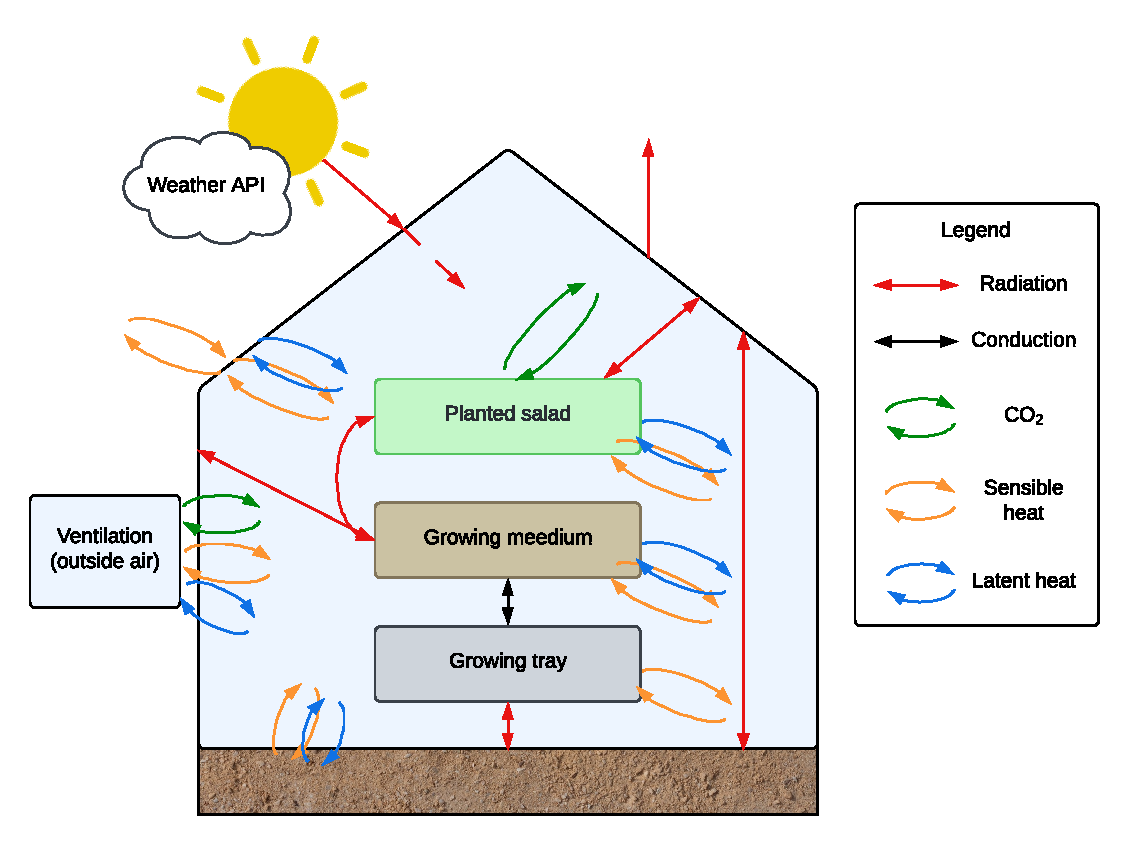
\includegraphics[width=.5\textwidth]{images/diagram.pdf}
    \caption{A simplified diagram of the heat, mass and CO\textsubscript{2} exchanges modelled within the framework. Image adapted from~\cite{rmward61_2019}.}\label{fig:diagram}
\end{figure}

\section{Nonlinear economic model predictive control}\label{sec:mpc}
A nonlinear economic model predictive control~(NEMPC) is adopted to maximize the profit from growing lettuce in a greenhouse. The objective of the proposed economic MPC for greenhouse control is to optimize the economic performance of the greenhouse system by controlling its actuators, such as heating, ventilation, and CO\textsubscript{2} injection. This is achieved by maximizing lettuce yield while minimizing operating costs over a finite prediction horizon. The nonlinear model predictive control framework incorporates the dynamics of the greenhouse and time-varying external conditions such as climate.

\subsection{System Dynamics}\label{subsec:mpc_dynamics}

The greenhouse system is modeled by a set of nonlinear state equations (see Section~\ref{sec:greenhouse}) that describe the evolution of the greenhouse states, such as temperature, humidity, and biomass. The discrete-time nonlinear system is given by:
\begin{equation}
	x(t+1) = f\left( x(t), u(t), \text{TVP}(t) \right),
\end{equation}
where \(x(t) \in \mathbb{R}^{n_x}\) represents the state vector at time step \(t\), \(u(t) \in \mathbb{R}^{n_u}\) represents the control input vector (actuators), and \(\text{TVP}(t)\) are time-varying parameters that include external climate conditions such as temperature, radiation, and humidity.

\subsection{Economic Objective Function}\label{subsec:mpc_objective}

The goal of the economic MPC is to maximize the revenue from lettuce production while minimizing the costs associated with actuator use. The objective function is composed of two terms: the profit from biomass, i.e.~the dry-weight of the lettuce, accumulation and the costs of actuators.

The revenue from lettuce production is proportional to the change in biomass between the initial state and the current state, expressed as:
\begin{equation}
	R(t) = P_L \cdot \frac{(x_{\mathrm{sdw}}(t) + x_{\mathrm{nsdw}}(t)) - (x_{0, \mathrm{sdw}} + x_{0, \mathrm{nsdw} })}{\rho_{dw}} \cdot A_c,
\end{equation}
where \(P_L\) is the price of lettuce per gram, \(A_c\) is the cultivated area, and \(x_{\mathrm{sdw}}\) and \(x_{\mathrm{nsdw}}\) are the biomass-related states.

In addition, the cost of operating the actuators at each time step is given by:
\begin{equation}
	C_u(t) = \sum_{i} \left( C_{\text{signal}}(u_i(t)) + C_{\text{CO2}}(u_i(t)) \right),
\end{equation}
where \(C_{\text{signal}}(u_i(t))\) is the cost associated with the actuator signal \(u_i(t)\) and \(C_{\text{CO2}}(u_i(t))\) represents the cost related to CO\textsubscript{2} emissions from the actuator.

Thus, the total cost at each time step is:
\begin{equation}
	l_t = -R(t) + C_u(t).
\end{equation}

\subsection{Optimization Problem Formulation}

The objective of the nonlinear economic MPC is to minimize the sum of the stage costs \(l_t\) over a finite prediction horizon \(N\), subject to system dynamics and constraints. The optimization problem is formulated as:
\begin{equation}
	\min_{\{u(t)\}_{t=0}^{N-1}} \sum_{t=0}^{N-1} l_t(x(t), u(t)),
\end{equation}
subject to:
\begin{align}
	x(t+1) &= f(x(t), u(t), \text{TVP}(t)), \\
	u_{\min} &\leq u(t) \leq u_{\max}, \quad \forall t = 0, \dots, N-1, \\
	x_{\min} &\leq x(t) \leq x_{\max}, \quad \forall t = 0, \dots, N, \\
	x(0) &= x_{\text{initial}}.
\end{align}
Here, \(x_{\min}\) and \(x_{\max}\) represent the bounds on the state variables, and \(u_{\min}\) and \(u_{\max}\) define the bounds on the control inputs, i.e., actuator signals.

\subsection{Time-Varying Parameters (TVP)}

The external climate conditions are modeled as time-varying parameters (TVP), which influence the system dynamics. These parameters include variables such as outdoor temperature, solar radiation, and humidity, and are provided by real-time climate data. These parameters are incorporated into the state equations, influencing the evolution of the greenhouse states.

\section{Results}
% Comparison of controlled greenhouse vs greenhouse without actuation
In the first set of simulations, we analyzed the non-linear behavior of the greenhouse under varying weather conditions and steps in actuation. We see how different actuations influence growth of structural and non-structural dry weight of the plant. The results in Figure~\ref{fig:steps} show that under given climate conditions, the influence of ventilation and humidification is insignificant on growth. Nevertheless, it has positive effect on convection and overall transfer of energy. Meanwhile, intense heating positive effects conversion of non-structural dry weight into structural but does not influence the overall non-structural dry weight buildup. CO\textsubscript{2} enrichment has a significant impact on non-structural plant growth.

\begin{figure*}[ht]
    \centering
    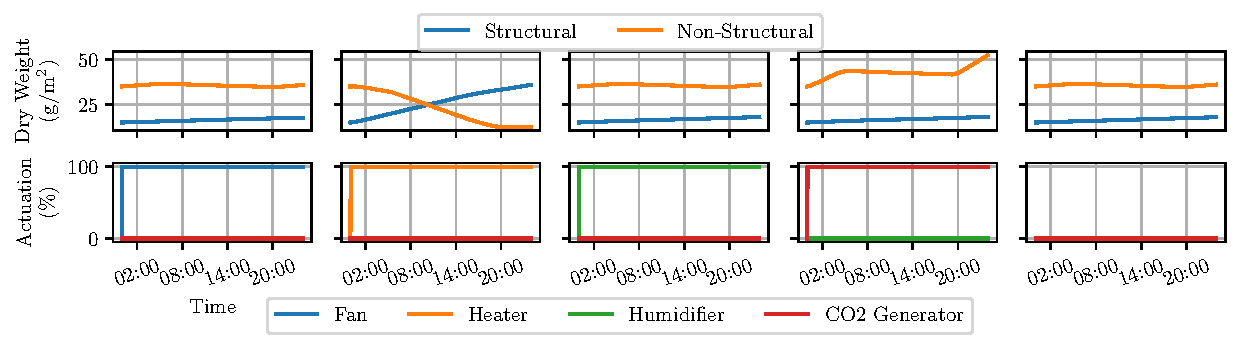
\includegraphics[width=\textwidth]{figures/step_response-outputs-2024-10-11_2024-10-26-120s.pdf}
    \caption{Responses of structural andd non-structural dry weight on step changes from off to maximum in following actuations from the left to the right: ventilation, heating, humidification, and CO\textsubscript{2} enrichment.}\label{fig:steps}
\end{figure*}


Second set of simulations compares the performance of the proposed NEMPC algorithm with a no control scenario. The parameters of NEMPC are as follows in Table~\ref{tab:parameters}. Results in Table~\ref{tab:comparison} demonstrate that the proposed economic MPC algorithm increased crop yield by 9\% and increase profit by more than 4\% in just 15 days of growth. The economic MPC algorithm also included social cost of carbon intensity of used energy sources, which reduced CO\textsubscript{2} consumption by 98\% while decreased the growth 4 times. We observe that there is a significant trade-off between the economic output and the carbon intensity of the energy sources. While our primal objective might be to maximize the economic output, we should also consider the environmental impact of our actions.

\begin{table}
    \centering
    \caption{Parameters of the NEMPC algorithm.}\label{tab:parameters}
    \begin{tabular}{lS[table-format=5.]l}
        \toprule
        Parameter & {Value} & Unit \\
        \midrule
        Prediction horizon & 10 & min \\
        Control horizon & 10 & min \\
        Number of steps & 10801 & --- \\
        Sampling time & 120 & s \\
        \bottomrule
    \end{tabular}
\end{table}

\begin{figure}\label{fig:control}
    \centering
    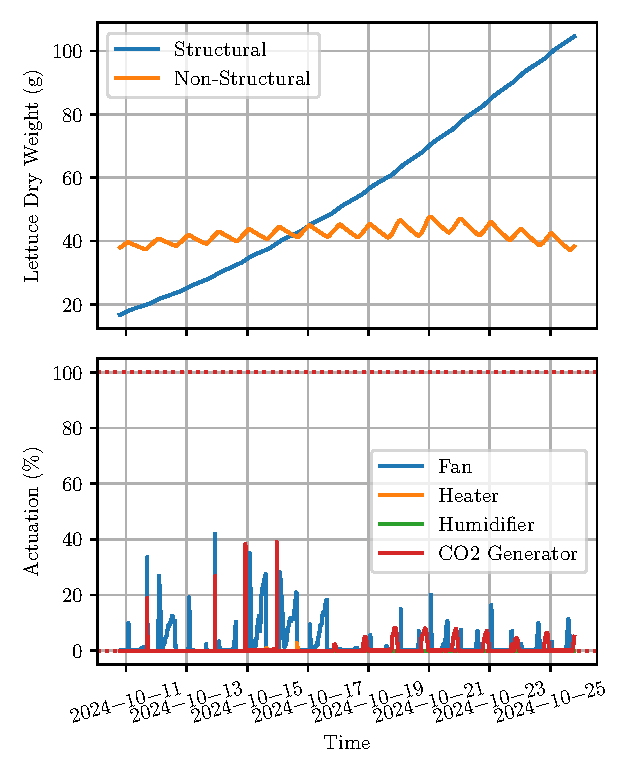
\includegraphics[width=.5\textwidth]{figures/greenhouse_control-mpc-N_5-steps_10801.pdf}
    \caption{A simplified diagram of the heat, mass and CO\textsubscript{2} exchanges modelled within the framework. Image adapted from~\cite{rmward61_2019}.}
\end{figure}

\begin{table}
    \centering
    \caption{Comparison of the NEMPC algorithm with a no control scenario.}\label{tab:comparison}
    \begin{tabular}{lS[table-format=4.2]S[table-format=4.2]S[table-format=4.2]}
        \toprule
        Parameter & {No control} & {NEMPC (CO\textsubscript{2})} & {NEMPC (\$)} \\
        \midrule
        Lettuce profit & 858.32 & 940.19 & 4120.63 \\
        Energy (Fan) & 0.00 & -0.03 & -0.16 \\
        Energy (Heater) & 0.00 & -0.45 & -21.68 \\
        Energy (Humidifier) & 0.00 & -0.05 & -0.00 \\
        Energy (CO2 Generator) & 0.00 & -9.95 & -697.59 \\
        CO2 (Fan) & 0.00 & -0.08 & -0.51 \\
        CO2 (Heater) & 0.00 & -1.48 & -70.84 \\
        CO2 (Humidifier) & 0.00 & -0.17 & -0.01 \\
        CO2 (CO2 Generator) & 0.00 & -32.52 & -2279.72 \\
        \midrule
        Total & 858.32 & 895.45 & 1050.12 \\
        \bottomrule
    \end{tabular}
\end{table}

% Educational trials
Educational trials on the interactive and user-friendly web interface for greenhouse design and ENMPC control pipeline revealed significant potential in increasing the understanding of non-linear control systems.

Via four layers of user customization of the greenhouse, participants grasped the main benefits of optimal control a d challenges related to non-linearity. The first layer is the greenhouse structure, where the user can select the shape of greenohouse affecting the energy exchange with the environment and suggested scaling of the actuation units. Second layer is the orientation and location of the greenhouse which affects the solar radiation and the weather conditions. Here we establish connection to weather and carbon intensity forecast APIs to provide real-time data along with forecasts and history replays. The third layer is the actuation units, where the user can overwrite the suggested scaling and select the actuators for the heating, ventilation, humidification, and CO\textsubscript{2} enrichment. Meanwhile the fourth layer is the control strategy, where the user can influence the control parameters, including the objective function and constrains of the economic MPC controller. While the user is customizing the greenhouse, the web interface provides real-time feedback. The user can also simulate the greenhouse operation over a selected period of time and analyze the results in terms of energy consumption, crop yield, and economic output.

\section{Conclusion}

\bibliographystyle{IEEEtran}
\bibliography{main}

\end{document}
